\pdfoutput=1
\pdfcompresslevel=9
\pdfinfo
{
    /Author (Autor)
    /Title (Tytuł pracy magisterskiej)
    /Subject (Bioinformatyka)
    /Keywords (DNAASM)
}
%\documentclass[a4paper,polish,onecolumn,oneside,floatssmall,11pt,titleauthor,wide,openright]{mwrep}
%\usepackage[scale={0.7,0.8},paper=a4paper,twoside]{geometry}
\documentclass[a4paper,onecolumn,twoside,openright,11pt,wide,floatssmall]{mwrep}
% \usepackage{polish}
\usepackage{amsmath}
\usepackage{amsfonts}
\usepackage{amssymb}
\usepackage{amsthm}
\usepackage{bookman}
\usepackage{algorithm}
\usepackage{algpseudocode}
\usepackage{geometry}
\usepackage{placeins}
%\usepackage{slashbox}
\usepackage[utf8x]{inputenc}
\usepackage[T1]{fontenc}
\usepackage{footnote}
\usepackage{enumerate}
% \usepackage{fancyvrb}
% \usepackage{t1enc}
% \usepackage[pdftex, bookmarks]{hyperref}
\usepackage[pdftex, bookmarks=false]{hyperref}

\floatname{algorithm}{Algorytm}
\renewcommand{\algorithmicforall}{\textbf{for each}}

\usepackage{caption}
%\usepackage[vlined]{algorithm2e}

\def\url#1{{ \tt #1}}

\usepackage{listings}
\usepackage{spverbatim}
\usepackage{enumitem}


\usepackage{fancyhdr}
\pagestyle{fancy}
\fancyhf{}
\fancyhead[CE,CO]{\leftmark}
\fancyfoot[LE,RO]{\thepage}
\usepackage[toc,page]{appendix}

\fancypagestyle{plain}{%
\fancyhf{}%
\fancyfoot[LE,RO]{\thepage}}

% marginesy
\textwidth\paperwidth
\advance\textwidth -55mm
\oddsidemargin-0.9in
\advance\oddsidemargin33mm
\evensidemargin0.9in
\advance\evensidemargin-33mm

\topmargin -1in
\advance\topmargin 25mm
\setlength\textheight{48\baselineskip}
\addtolength\textheight{\topskip}
\marginparwidth15mm

\clubpenalty=10000 % to kara za sierotki
\widowpenalty=10000 % nie pozostawia wdów
\brokenpenalty=10000 % nie dzieli wyrazów pomiędzy stronami
\sloppy

\tolerance4500
\pretolerance250
\hfuzz=1.5pt
\hbadness1450

\linespread{1.5} %interlinia
% ŻYWA PAGINA
\renewcommand{\chaptermark}[1]{\markboth{\scshape\small\bfseries \
#1}{\small\bfseries \ #1}}
\renewcommand{\sectionmark}[1]{\markboth{\scshape\small\bfseries\thesection.\
#1}{\small\bfseries\thesection.\ #1}}
\renewcommand{\headrulewidth}{0.5pt}
\renewcommand{\footrulewidth}{0.pt}
%%\pagestyle{uheadings}

\usepackage[pdftex]{color,graphicx}
\usepackage[polish]{babel}

% \textheight232mm
% \setlength{\textwidth}{\textwidth}
% \setlength{\oddsidemargin}{\evensidemargin}
% \setlength{\evensidemargin}{0.3cm}
\usepackage[sort, compress]{cite}
\usepackage{setspace}

\definecolor{orange}{rgb}{1,0.5,0}

% definicje komand todo
\newcommand\todo[1]{\textcolor{red}{#1}}
\newcommand\przeredagowac[1]{\textcolor{orange}{#1}}
\newcommand\info[1]{\textcolor{blue}{#1}}

%\usepackage{multibib}
%\newcites{bk,st,doc,web}{Książki i~artykuły,Standardy i~zalecenia,Dokumentacja produktów,Publikacje i~serwisy internetowe}

\theoremstyle{definition}
\newtheorem{defn}{Definicja}[chapter]
\newtheorem{conj}{Teza}[section]
\newtheorem{conjmain}{Teza}
\newtheorem{exmp}{Przykład}[chapter]

\theoremstyle{plain}% default
\newtheorem{thm}{Twierdzenie}[section]
\newtheorem{lem}[thm]{Lemat}
\newtheorem{prop}[thm]{Hipoteza}
\newtheorem*{cor}{Wniosek}

\theoremstyle{remark}
\newtheorem*{rem}{Uwaga}
\newtheorem*{note}{Uwaga}
\newtheorem{case}{Przypadek}[chapter]

\definecolor{ListingBackground}{rgb}{0.95,0.95,0.95}

\begin{document}

% kody źródłowe wplatane w tekst
\lstdefinestyle{incode}
{
basicstyle={\footnotesize},
keywordstyle={\bf\footnotesize\color{blue}},
commentstyle={\em\footnotesize\color{magenta}},
numbers=left,
stepnumber=5,
firstnumber=1,
numberfirstline=true,
numberblanklines=true,
numberstyle={\sf\tiny},
numbersep=10pt,
tabsize=2,
xleftmargin=17pt,
framexleftmargin=3pt,
framexbottommargin=2pt,
framextopmargin=2pt,
framexrightmargin=0pt,
showstringspaces=true,
backgroundcolor={\color{ListingBackground}},
extendedchars=true,
% title=\lstname,
captionpos=b,
% abovecaptionskip=1pt,
% belowcaptionskip=1pt,
frame=tb,
framerule=0pt,
}

% kody źródłowe z podpisem
\lstdefinestyle{outcode}
{
basicstyle={\footnotesize},
keywordstyle={\bf\footnotesize\color{blue}},
commentstyle={\em\footnotesize\color{magenta}},
numbers=left,
stepnumber=5,
firstnumber=1,
numberfirstline=true,
numberblanklines=true,
numberstyle={\sf\tiny},
numbersep=10pt,
tabsize=2,
xleftmargin=17pt,
framexleftmargin=3pt,
framexbottommargin=2pt,
framextopmargin=2pt,
framexrightmargin=0pt,
showstringspaces=true,
backgroundcolor={\color{ListingBackground}},
extendedchars=true,
% title=\lstname,
captionpos=b,
% abovecaptionskip=1pt,
% belowcaptionskip=1pt,
frame=tb,
framerule=0.1pt,
}

%\counterwithin{exmp}{chapter}
%\counterwithout{exmp}{section}
\renewcommand*\lstlistingname{Wydruk}
\renewcommand*\lstlistlistingname{Spis wydruków}

\pagenumbering{roman}
\renewcommand{\baselinestretch}{1.0}
\raggedbottom

% todo odkomentować strony tytulowe !
% 
\begin{titlepage}
    % Strona tytułowa


    % Życiorys
    \newpage\thispagestyle{empty}
    \begin{tabular}{p{5cm} p{12cm}}
    \begin{minipage}{5cm}
    \center
    %% \includegraphics[height=6.5cm,width=4.5cm]{img/ja.png}
    \end{minipage}
    &
    \begin{minipage}{12cm}
    \begin{flushleft}
    \par\noindent\vspace{0\baselineskip}
    \begin{tabular}[h]{l l}
    {\normalsize\it Specjalność:} & Informatyka -- \\
    & Systemy Informacyjno Decyzyjne \\
    \end{tabular}
    \par\noindent\vspace{1\baselineskip}
    \begin{tabular}[h]{l l}
    {\normalsize\it Data urodzenia:} & {\normalsize 03.04.1992}
    \end{tabular}
    \par\noindent\vspace{1\baselineskip}
    \begin{tabular}[h]{l l}
    {\normalsize\it Data rozpoczęcia studiów:} & {\normalsize 20.02.2016}%1 października 2012 r.}
    \end{tabular}
    \par\noindent\vspace{1\baselineskip}
    \end{flushleft}
    \end{minipage}
    \end{tabular}
    \vspace*{0\baselineskip}
    \begin{center}
	{\large\bfseries Życiorys}\par\bigskip
    \end{center}
	\mockup{
	Urodziłem się 3 kwietnia 1992 roku w~Kielcach. W~2008 roku rozpocząłem naukę w~II Liceum Ogólnokształcącym im. Jana Śniadeckiego w~Kielcach, w~klasie o~podstawie programowej w~zakresie rozszerzonym z~matematyki, informatyki, fizyki i~astronomii . W~2011 roku uzyskałem wykształcenie średnie oraz świadectwo dojrzałości... 
	}
    \indent

    \par
    \vspace{2\baselineskip}
    \hfill\parbox{15em}{{\small\dotfill}\\[-.3ex]
    \centerline{\footnotesize podpis studenta}}\par
    \vspace{1\baselineskip}
    \begin{center}
 	{\large\bfseries Egzamin dyplomowy} \par\bigskip\bigskip
    \end{center}
    \par\noindent\vspace{1.0\baselineskip}
    Złożył egzamin dyplomowy w dn. \dotfill
    \par\noindent\vspace{1.0\baselineskip}
    Z wynikiem \dotfill
    \par\noindent\vspace{1.0\baselineskip}
    Ogólny wynik studiów \dotfill
    \par\noindent\vspace{1.0\baselineskip}
    Dodatkowe wnioski i uwagi Komisji \dotfill
    \par\noindent\vspace{1.0\baselineskip}
    \dotfill

    % Streszczenie po polsku
    \newpage\thispagestyle{empty}
    \vspace*{2\baselineskip}
    \begin{center}
	{\large\bfseries Streszczenie}\par\bigskip
	\vspace*{2\baselineskip}
    \end{center}

    \itshape
    \todo{todo}
    \vspace*{3\baselineskip}

    \noindent{\bf Słowa kluczowe}: {\itshape \todo{todo.}}
    %\par
    %\vspace{4\baselineskip}
    
    % Streszczenie po angielsku
    \newpage\thispagestyle{empty}
    \vspace*{2\baselineskip}
    \begin{center}
	{\large\bfseries Abstract}\par\bigskip
	\vspace*{2\baselineskip}
    \end{center}
    \noindent{\bf Title}: {\itshape \todo{XXX}}\par
    \vspace*{1\baselineskip}
    \itshape
    \todo{XXX}
    \vspace*{3\baselineskip}

    \noindent{\bf Key words}: {\itshape \todo{XXX}.}

\end{titlepage}

% ex: set tabstop=4 shiftwidth=4 softtabstop=4 noexpandtab fileformat=unix filetype=tex spelllang=pl,en spell:


%\newpage\null\thispagestyle{empty}\newpage

% % Podziękowania
\newpage\thispagestyle{empty}



\tableofcontents
% \addcontentsline{toc}{chapter}{{Przedmowa1}{vii}}{vii}

% \chapter*{Spis tablic, rysunków i~wydruków}
% \listoftables
% \listoffigures
% \listofalgorithms
% \lstlistoflistings

%\setlength{\baselineskip}{7mm}
\newpage
\pagenumbering{arabic}
\raggedbottom{}

%\setcounter{page}{1}
\setcounter{tocdepth}{1}



\chapter{Wstęp}
\label{section:wstep}

\section{Cel i zakres pracy}
\label{section:cel_i_zakres_pracy}

\subsection{Hipotezy}

\begin{enumerate}[I.]
	\item \textit{
		Można zaproponować strukturę bazy danych do przechowywania danych opisujących genomy, taką że będzie ona elastyczna, łatwa w modyfikacji, uniezależniona od semantyki przechowywanych struktur biologicznych.
		} \\
	\todo{krótki opis}
	
	\item \textit{
		Można dostarczyć abstrakcję widoków na dane genetyczne, umożliwiające analizę danych z różnych perspektyw w kontekście licznych zbiorów
		danych genetycznych.
		} \\
	\todo{krótki opis}
	
	\item \textit{
		Można dostarczyć aplikację do przechowywania i analizy genomów, która w~przystępny sposób umożliwi przeglądanie sekwencji genetyczych bez konieczności posiadania wydajnej maszyny klienckiej. 
		} \\
	\todo{krótki opis}
	
\end{enumerate}

\subsection{Plan badań}
-genom ogorka \\
-baza danych generycza \\
-algorytmy \\
-wygoda uzytkownika \\
-wydajne przegladanie \\

\section{Układ pracy}
\label{section:uklad_pracy}

\section{Przegląd literatury}

\chapter{Sekwencjonowanie i adnotacja genomu}
\label{section:sekwencjonowanie_i_adnotacja}

\subsection*{Centralny dogmat bioinformatyki}
Podstawowym założeniem w bioinformatyce jest następująca zależność:
Informacja, która jest zawarta w sekwencji nukleotydowej przekłada się na strukturę przestrzenną białek i innych cząsteczek, które są w genomie zakodowane. 
Dzięki odpowiednio uformowanej strukturze przestrzennej, białka stają się aktywne i mogą oddziaływać w przestrzeni komórkowej, pełniąc różne funkcje molekularne i angażując się w procesy biochemiczne. 
Funkcją biochemiczną może być np. reakcja w którą wchodzi dane białko łącząc się z inną substancją. 
Efekt końcowy oddziaływań zbioru wybranych białek obserwujemy w postaci np. wyglądu zewnętrznego (fenotypu), zachowania lub funkcjonowania organizmu.

Chcąc posiąść wiedzę na temat funkcjonowania organizmu, fenotypu oraz cech odmian, w których występują różnego rodzaju mutacje wpływające na ich unikatowość w pierwszym etapie należy określić geny jakie w tym organiźmie występują oraz zmienność pomiędzy analizowanymi osobnikami.
Proces poznania sekwencji genów (i białek) jest etapem, w którym opracowano dość dobrze procedury eksperymentalne. 
Po uzyskaniu danych należy przeprowadzić adnotację strukturalną i funkcjonalną w celu określenia roli jaką dany gen a w dalszej kolejności kodowane białko spełnia w komórce. 
Dąży się do ustalenia struktury przestrzennej białka, domen wpływających na aktywność enzymatyczną lub budulcową oraz klasyfikacji ontologicznej według kategorii takich jak proces biologiczny, funkcja molekularna czy lokalizacja w komórce.

\begin{figure}[h]
	\centering
	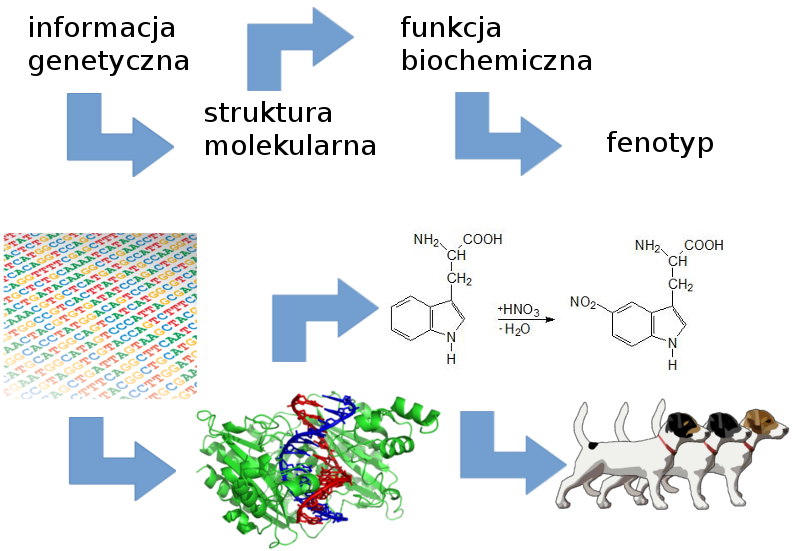
\includegraphics[width=0.9\textwidth]{img/centralny-dogmat.png}
	\caption{Centralny dogmat bioinformatyki}
	\vspace{-0.5cm}
	\caption*{\scriptsize Źródła: 
		\url{http://www.wikiwand.com/en/DNA},
		\url{http://igoscience.com/dna-sequence-genetic-code/} \\
		\url{https://commons.wikimedia.org/wiki/File\%3AReakcja\_ksantoproteinowa\_dla\_tryptofanu.jpg}, \\
		\url{https://www.russell-terrier.org/index.php/blog/56-maść-jrt-i-prt-w-praktyce-część-vi-fenotyp}
	}
	\label{img:centralny-dogmat}
\end{figure}

\subsection*{Problemy bioinformatyki}
Bioinformatyka, jest to bardzo prężnie rozwijająca się nauka i jak każda dziedzina naukowa boryka się z pewnymi problemami.
Jednym z nich jest mnogość otrzymywanych danych, ich scalanie i deponowanie.
Inny problem dotyczący baz danych polega na tym, że wiele baz powstaje jako wynik grantu badawczego a potem z tymi danymi często nic się nie dzieje.

,,Podstawowe bazy'' są tworzone i z powodzeniem wykorzystywane do naukowych doświadczeń.
Takie bazy danych mają często kuratorów oceniających istotność i mają tzw. zbiory referencyjne - stanowią standard.
Każdego dnia ludzkość poznaje tysiące nowych sekwencji, które są deponowane w cyfrowych przechowalniach, tworząc tzw. ,,wtórne bazy danych'', które nim znajdą się w bazach ustandaryzowanych muszą być przeanalizowane pod różnym kątem w zależności od celu doświadczeń i często zawierają dodatkowe pośrednie elementy, których nie zamieszcza się w bazach głównych.
Bazy wtórne gromadzą najczęściej zbiór informacji pochodzący z różnych źródeł.
Niejednokrotnie zdarza się, że do bazy pierwotnej są wprowadzane modyfikacje, które nie zostają już uwzględnione w późniejszych bazach wtórnych. 
Taka niespójność wprowadzania danych generuje w nich błędy, co utrudnia pracę w kolejnych realizowanych projektach.

Często bioinformatyczne bazy danych powstają jako wynik prac badawczych (grantów).
Po zakończeniu projektu takie bazy danych nie są pielęgnowane, co sprawia, że dane się dezaktualizują.
Jedną z przyczyn jest brak dominującego standardu.

Następnym utrudnieniem jest problem techniczny dotyczący ogromnego rozmiaru danych.
Sekwencja przykładowego genomu człowieka zajmuje ponad 3GB, natomiast opis samego eksperymentu sekwencjonowania może zająć nawet kilkaset gigabajtów. 
Okazuje się, że często laboratorium ponownie przeprowadza eksperyment sekwencjonowania zamiast uwzględnić dane zebrane poprzednio. Przyczyną może być zbyt mały udział informatyków w ośrodkach wykonujących takie badania.

Kolejnym problemem jest mnogość standardów. 
Często rozwiązania projektowane są od podstaw w każdym ośrodku niezależnie.
Takie podejście skutkuje tym, że dla pojedynczego zadania, mamy kilkanaście bądź kilkadziesiąt różnych metod, które nie koniecznie są ze sobą kompatybilne. 
Innym problemem, z jakim zmagają się biolodzy przy analizie danych jest to, że wyjście jednego programu nie jest kompatybilne z wejściem drugiego programu, który potrzebują aktualnie wykorzystać. 
Próby rozwiązania takiego kłopotu skutkują często zdefiniowaniem kolejnego standardu, co może jeszcze bardziej skomplikować sytuację jeśli nowy sposób nie zostanie przyjęty przez większe grono naukowców.

%-niekontynuowane projekty \\
%-dane bazują na eksperymentach, błędy propagujące się \\
%-wiele różnych standardów, niekompatybilne \\
%-nieinformatyczni biolodzy \\
%-sposoby finansowania nauki \\

\section{Sekwencjonowanie i assembling DNA}
Sekwencjonowanie to jedna z technik biologii molekularnej, pozwalająca na odczytanie kolejności nukleotydów w cząsteczce DNA.

Najlepiej byłoby, gdyby efektem projektu poznania genomu była możliwość przedstawienia kompletnej sekwencji nukleotydowej w sposób przyjęty w naukach biologicznych, tzn. hierarchiczny, gdzie genom składa się z chromosomów, zaś chromosomy są to ciągłe sekwencje symboli.
Dodatkowo na chromosomach wprowadzamy adnotacje, zawierające istotne informacje o podsekwencjach np. geny, struktury genów, funkcje.
Jednak w rzeczywistości, pojawia się wiele potencjalnych problemów związanych z takim opisem.
Proces sekwencjonowania nie jest doskonały, nie dostarcza ciągłych sekwencji chromosomów.
Materiał (DNA) jest różny dla różnych osobników tego samego gatunku. 
Nie istnieje jedna sekwencja dla gatunku z powodu indywidualnej zmienności genetycznej jednostek. 
Nawet komórki tego samego osobnika mogą różnić się w zawartości genetycznej z powodu mutacji somatycznych. 
Złożony genom będzie jedną, konkretną reprezentacją zmienności występującej u danego gatunku. 
Zasadniczo sekwencjonuje się tylko jednego osobnika, ale czasami genom stanowi konsensus wielu połączonych próbek (projekt HUGO). 
Dodatkowo procesowi sekwencjonowania zawsze będą towarzyszyć błędy na poziomie poszczególnych nukleotydów oraz ich kolejności (błędy techniki sekwencjonowania i assemblingu).
Każdy złożony genom jest wynikiem serii złożeń krótszych odczytów metodami heurystycznymi i powinien być traktowany jako roboczy ,,draft''.

\begin{figure}[h]
	\centering
	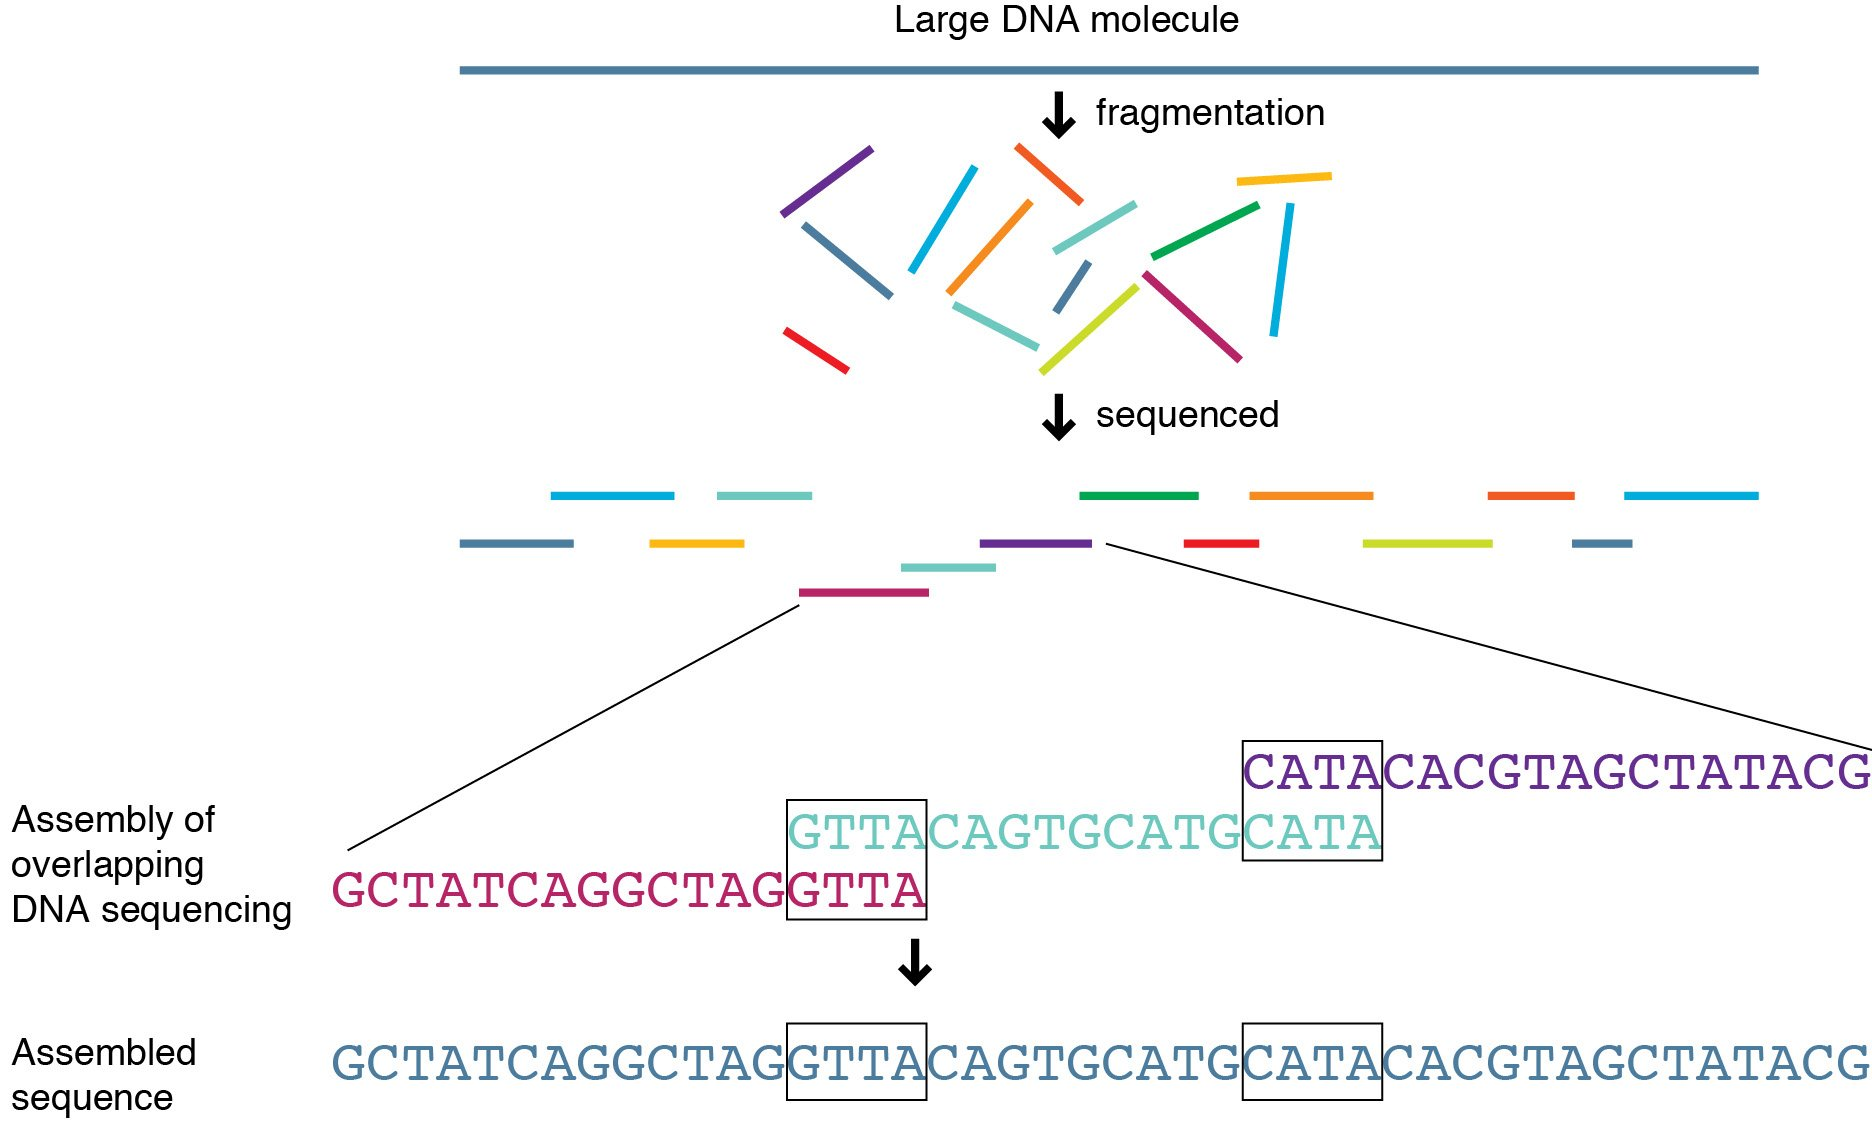
\includegraphics[width=0.9\textwidth]{img/sequenctioning-process.png}
	%zdjecie z %http://knowgenetics.org/whole-genome-sequencing/
	\caption{Schemat sekwencjonowania}
	\vspace{-0.5cm}
	\caption*{\scriptsize Źródło: \url{http://knowgenetics.org/whole-genome-sequencing/}}
	\label{img:schemat-sekwencjonowania}
\end{figure}

W większości projektów sekwencjonowania w pierwszym etapie następuje losowe pocięcie DNA na bardzo małe fragmenty.
W zależności od wykorzystanej technologii, fragmenty mogą mieć różną długość.
Istnieje trend w kierunku uzyskiwania odczytów technikami dającymi coraz dłuższe fragmenty np. technika PacBio czy Oxford Nanopore - ale są one obarczone dość dużym błędem. 
Tradycyjne sposoby (Sanger) dawały fragmenty długości około 1000 par zasad. Obecnie wykorzystywane techniki dające najkrótsze rezultaty osiągają wyniki rzędu dziesiątek pz. (SOLiD, Illumina - rys.\ref{img:sekwencjoner-illumina}).

\begin{figure}[h]
	\centering
	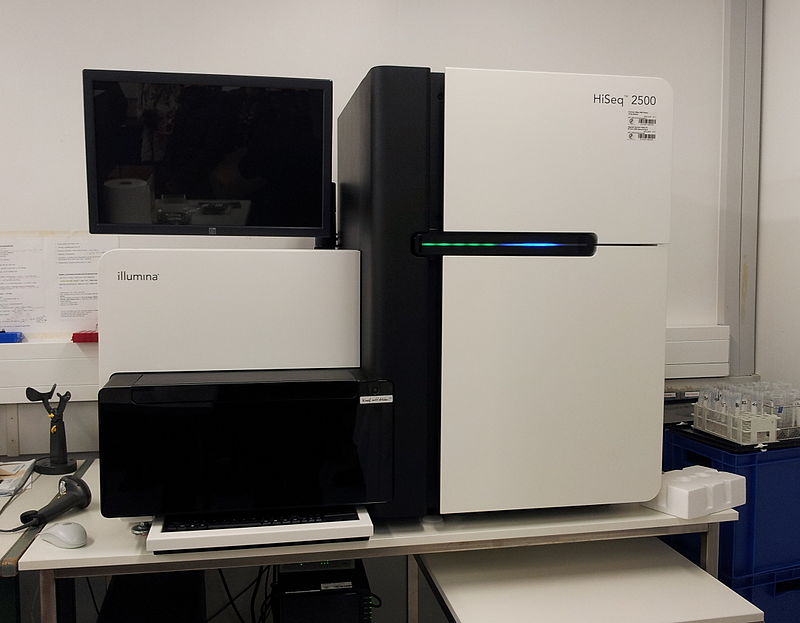
\includegraphics[width=0.75\textwidth]{img/sekwencjoner-illumina.jpg}
	%zdjecie z http://wiedza.alkahest.umcs.pl/jak-limfocyty-t-przekazuja-informacje/
	\caption{Sekwencjoner Illumina HiSeq 2500}
	\vspace{-0.5cm}
	\caption*{\scriptsize Źródło: \url{http://wiedza.alkahest.umcs.pl/jak-limfocyty-t-przekazuja-informacje/}}
	\label{img:sekwencjoner-illumina}
\end{figure}

Następie, w procesie assemblingu, fragmenty sekwencji są składane w dłuższe odcinki.
Dobór algorytmu jest zależny od długości zsekwencjonowanych odcinków.
Jest to proces skomplikowany i wykorzystywane są do tego zasobożerne programy. 
Efektem początkowego składania sekwencji są kontigi.
Na dalszych etapach, po analizach wykorzystujących biblioteki dłuższych sekwencji DNA, kontigi są zespalane w struktury zwane skafoldami.
Mają one zazwyczaj postać sekwencji z lukami o znanej długości - dziury oznaczane są znakiem ,,N''.

\section{Adnotacje}
Aby wykorzystać cały potencjał sekwencji genomu, musi on zostać opatrzony adnotacjami, które zawierają istotne informacje z biologicznego punktu widzenia.
Kompletna adnotacja genomu stanowi duże wyzwanie dla biologów, a jej wyniki są w dużej mierze uzależnione od jakości złożenia genomu w procesie assemblingu i otrzymanych odczytów po sekwencjonowaniu.

Adnotacja genomu jest procesem odnalezienia regionów kodujących, zidentyfikowania genów oraz określenia funkcji jakie pełnią.
Adnotacją możemy nazywać np. przypis będący notatką dodaną jako wyjaśnienie bądź komentarz. Dzielą się na przypisy:
\itemize{
	\item strukturalne (identyfikacja obiektów genomowych)
	\item funkcjonalne (biologiczne informacje związane z obiektami genomowymi)
}
\\
Proces adnotacji można podzielić na 3 główne fazy:
\enumerate{
	\item Identyfikacja niekodujących fragmentów.
	\item Przewidywanie genów.
	\item Dołączenie biologicznych informacji.
}\\

Większość technik wykorzystuje narzędzia oparte o wyszukiwanie homologicznych sekwencji używając do tego celu publiczne bazy danych genomów.
Przewidywanie genów to czynność mająca na celu zidentyfikowanie fragmentów DNA, które odpowiedzialne są za kodowanie białek.
Wśród organizmów zbudowanych z komórek posiadających jądro komórkowe z chromosomami (eukarioty), odcinki kodujące sekwencję aminokwasów nazywane są eksonami, które zazwyczaj oddzielone są fragmentami niekodującymi - intronami (rys.\ref{img:intron-exon}).

\begin{figure}[h]
	\centering
	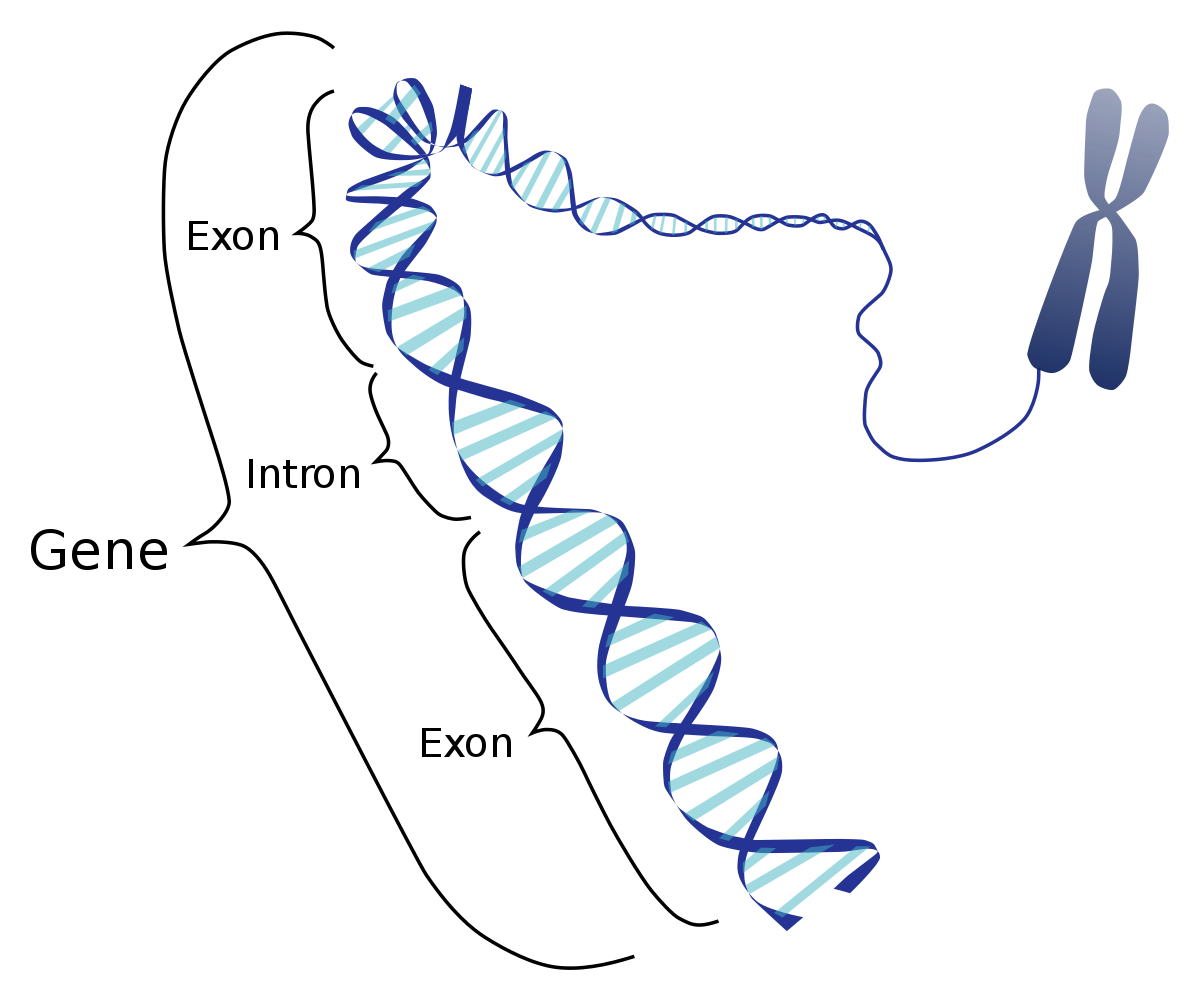
\includegraphics[width=0.75\textwidth]{img/intron-exon.png}
	\caption{Reprezentacja intronów i eksonów z genem zawierającym pojedynczy intron i dwa eksony.}
	\vspace{-0.5cm}
	\caption*{\scriptsize Źródło: \url{https://en.wikipedia.org/wiki/File:Gene\_Intron\_Exon\_nb.svg}}
	\label{img:intron-exon}
\end{figure}


\section{Prezentacja danych}
Kolejnym etapem projektu poznania genomu jest zazwyczaj umieszczenie go w przeglądarce genomów wraz z adnotacjami. Są to programy mające wygodny interfejs graficzny, gromadzące i w przystępny sposób prezentujące informacje uzyskane w poprzednich etapach badań. Dzięki nim naukowcy mają możliwość przede wszystkim łatwego dostęp do danych, a także posiadają wygodne narzędzie do dalszych prac. 
Ważnym aspektem jest fakt, że dzięki przeglądarkom mogą dzielić się wynikami prac z innymi zespołami badawczymi, bez czego postęp biotechnologiczny rozwijałby się znacznie wolniej.

Dane wizualizowane są najczęściej w sposób interaktywny pozwalając na obserwację genomu z perspektyw makro (chromosomów) i mikro (poszczególne geny, ciągi nukleotydowe).

Udostępnienie genomu umożliwia rozpoczęcie wielu prac z zakresu jego szczegółowej analizy, poczynając od analizy struktury i funkcji genów a kończąc na analizach filogenetycznych obejmujących całe genomy. 
Celem analiz filogenetycznych jest rekonstrukcja historii ewolucji  organizmów. W klasycznym podejściu historia ewolucji jest odtwarzana na podstawie porównań cech morfologicznych i fizjologicznych badanych organizmów.
Filogenetyka molekularna rekonstruuje związki filogenetyczne między badanymi sekwencjami, opierając się na założeniu, iż sekwencje przodka mutują w sekwencje potomków a podobne gatunki są genetycznie blisko spokrewnione.
Powszechnym przykładem wykorzystania udostępnionego genomu jest analiza sekwencji, na której badacz projektuje inne sekwencje np. startery do PCR, czy startery do RT-PCR\footnote{metoda stosowana do ilościowego określania ekspresji specyficznych genów, również w diagnostyce medycznej i mikrobiologicznej.}.


\section{Przegląd literatury - istniejące rozwiązania}

\subsection*{Najpopularniejsze przeglądarki}
\begin{itemize}
	% https://en.wikipedia.org/wiki/UCSC_Genome_Browser
	% http://genome.ucsc.edu/
	\item \href{https://genome.ucsc.edu}{\emph{UCSC browser}} (rys.\ref{img:przegladarka-UCSC}) \label{przegladarka-UCSC}
	
	przeglądarka on-line, opracowana na Uniwersytecie Kalifornijskim w~Santa Cruz w 2000 roku; główni autorzy - Jim Kent, David Haussler; zaimplementowana w~większości w~języku~C. Udostępniana darmowo dla akademickich zastosowań, dla komercyjnych wymagana licencja \emph{Kent Informatics}. Zawiera 46 gatunków organizmów. Pozwala wyświetlać sekwencje o dowolnym rozmiarze - od pojedynczych zasad po chromosomy. Badacze mogą wyświetlać własne dane i wyświetlać je w kontekście referencyjnego genomu. Widoki tworzone przez użytkowników mogą być udostępniane innym użytkownikom.
	
	W porównaniu do CuGene:
	brak funkcjonalności widoków z priorytetyzacją nakładających się na siebie typów danych. Brak algorytmów wyszukiwania Knutha-Morrisa-Pratta i Smitha-Watermana. Skomplikowane narzędzie, trudne dla początkujących użytkowników.
	\begin{figure}[h]
		% https://en.wikipedia.org/wiki/UCSC_Genome_Browser#/media/File:BrowserFoxp2.jpg
		\centering
		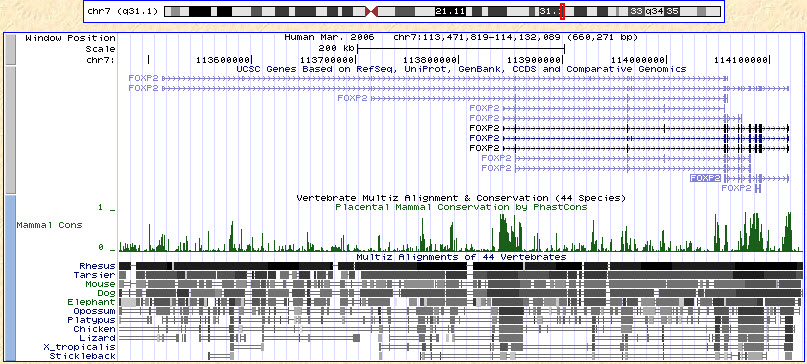
\includegraphics[width=0.75\textwidth]{img/browser-UCSC.jpg}
		\caption{Przeglądarka UCSC.}
		\vspace{-0.5cm}
		\caption*{\scriptsize Źródło: \url{https://en.wikipedia.org/wiki/UCSC\_Genome\_Browser\#/media/File:BrowserFoxp2.jpg}}
		\label{img:przegladarka-UCSC}
	\end{figure}
	
%%%%%%%%%%%%%%%%%%
	\item \href{http://gbrowse.org}{\emph{Gbrowse}} (rys.\ref{img:przegladarka-gbrowse})
	\label{przegladarka-Gbrowse}
	% http://gmod.org/wiki/GBrowse
	
	projekt napisany w Pearlu, przeglądarka on-line; powstała w 2002 roku; funkcjonuje na licencjach \textit{GPL 2.0} oraz \textit{Artistic Licence 2.0}; wielojęzykowa; aktywnie wspierana i wykorzystywana, jedna z najpopularniejszych, aczkolwiek w czasie pisania pracy, główna strona projektu (\textit{http://gbrowse.org/}) była nieosiągalna. Pozwala m.in. na tworzenie linków do dowolnych adnotacji, nawigację poprzez przewijanie, przybliżanie, wspiera format danych GFF, zapamiętuje ustawienia użytkownika podczas trwania sesji. Łączy się z różnymi publicznymi bazami danych (\textit{BioSQL}, \textit{Chado}) Na tle innych przeglądarek wyróżnia się architekturą umożliwiającą wykorzystanie edytowalnych pluginów firm trzecich.
	\begin{figure}[h]
		% http://gmod.org/mediawiki/images/1/10/GBrowse_screenshot1.png
		\centering
		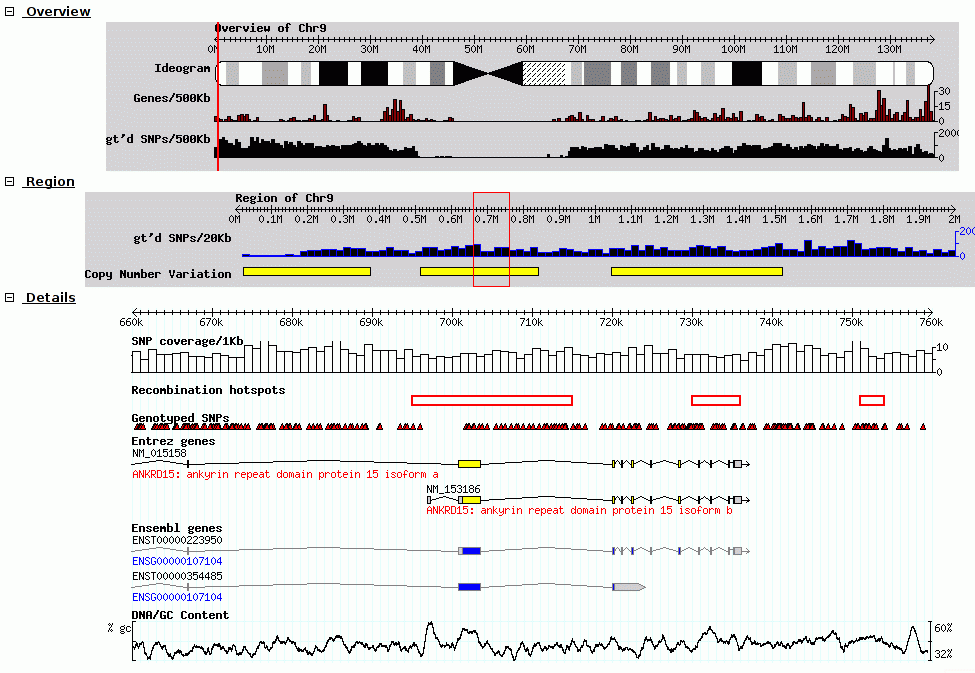
\includegraphics[width=0.75\textwidth]{img/browser-gbrowse.png}
		\caption{Przeglądarka GBrowse.}
		\vspace{-0.5cm}
		\caption*{\scriptsize Źródło: \url{http://gmod.org/mediawiki/images/1/10/GBrowse\_screenshot1.png}}
		\label{img:przegladarka-gbrowse}
	\end{figure}
	
	W porównaniu do CuGene:
	brak funkcjonalności widoków z priorytetyzacją nakładających się na siebie typów danych. Brak algorytmów wyszukiwania Knutha-Morrisa-Pratta i Smitha-Watermana.	
	\\
	
%%%%%%%%%%%%%%%%
	\item \href{http://www.ensembl.org}{\emph{ENSEMBL}} \label{przegladarka-ENSEMBL} (rys.\ref{img:przegladarka-ensembl})
	% http://www.ensembl.info/about/
	% https://en.wikipedia.org/wiki/European_Bioinformatics_Institute
	
	projekt rozpoczęty w celu opisania genomu człowieka i~udostępnienia go w sieci w 1999 roku. Powstał we współpracy pomiędzy EMBL-EBI\footnote{EBI (ang. European Bioinformatics Institute), jest częścią EMBL (ang. European Molecular Biology Laboratory)} a WSI\footnote{WSI (ang. Wellcome Sanger Institute)}. W projekcie uczestniczy 8 zespołów - łącznie około 50 członków. Udostępnione genomy są w większości takie jak w przelgądarce UCSC. Udostępnia API pozwalające pisać samodzielnie skrypty do pozyskiwania interesujących porcji danych.
	
	Zasadniczą różnicą w porównaniu do CuGene jest struktura bazy danych. W projekcie ENSEMBL zastosowano klasyczne podejście polegające na zaprojektowaniu bazy w formie niegenerycznej, odzwierciedlającej biologiczne obiekty w naturze. Na diagramie bazodanowym (rys.\ref{img:db-ensebl}) widać takie tabele jak markery, eksony, transkryptomy, allele, geny itd.
	%https://www.ensembl.org/info/docs/api/core/features_analyses_core.pdf
	
	\begin{figure}[h]
		% https://en.wikipedia.org/wiki/File:Ensembl_release58_sgcb_screenshot.png
		\centering
		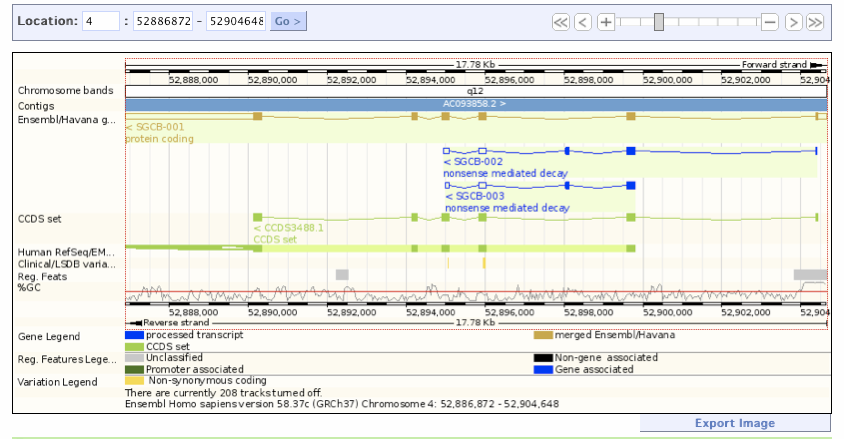
\includegraphics[width=0.75\textwidth]{img/browser-ensembl.png}
		\caption{Przeglądarka EMSEMBL.}
		\vspace{-0.5cm}
		\caption*{\scriptsize Źródło: \url{https://en.wikipedia.org/wiki/File:Ensembl\_release58\_sgcb\_screenshot.png}}
		\label{img:przegladarka-ensembl}
	\end{figure}
	\begin{figure}[h]
		% https://www.ensembl.org/info/docs/api/core/core_schema.html
		\centering
		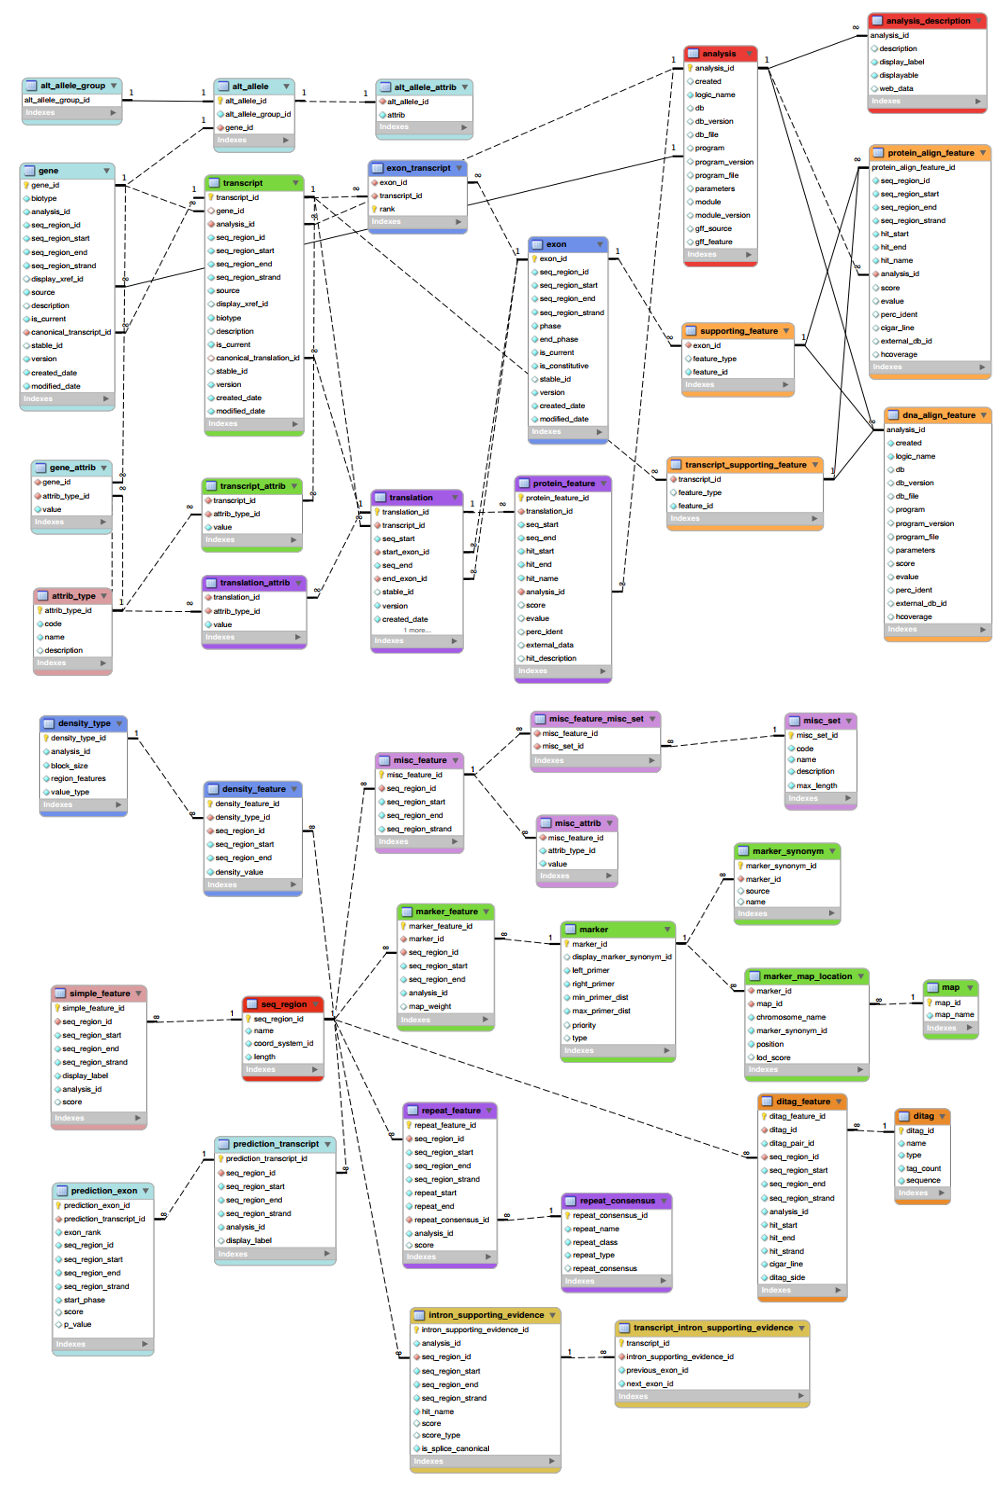
\includegraphics[width=1\textwidth]{img/db-ensembl.png}
		\caption{Fragment schematu bazdy danych EMSEMBL.}
		\vspace{-0.5cm}
		\caption*{\scriptsize Źródło: \url{https://www.ensembl.org/info/docs/api/core/core\_schema.html}}
		\label{img:db-ensebl}
	\end{figure}
		
%%%%%%%%%%%%%%%
	\item \href{http://bioviz.org/igb/index.html}{\emph{IGB}} \label{IGB}
	(rys.\ref{img:przegladarka-igb})
	% https://en.wikipedia.org/wiki/Integrated_Genome_Browser
	% https://bitbucket.org/lorainelab/genoviz-sdk/src
	% https://sourceforge.net/projects/genoviz/
	
	%Integrated Genome Browser to projekt rozpoczęty przez firmę \emph{Affymetrix}, jednak porzucony przez nią i~rozwijany w~środowisku akademickim. Przeglądarka napisana w~Javie, obecnie na prawach Academic free license.
	
	Integrated Genome Browser to projekt używany przez wiele uniwersytetów na całym świecie. Zapoczątkowany przez \emph{Affymetrix}, jednak od 2004 roku jego kod został upubliczniony. Ostatnie wiadomości\footnote{\url{http://bioviz.org/igb/news.html}} odnośnie rozwoju projektu publikowane były w połowie 2016 roku. Oparty na platformie \textit{GenoViz}\footnote{\url{https://sourceforge.net/projects/genoviz/}} dostarczającej re-używalnych komponentów do wizualizacji danych genetycznych. Rozwój platformy zatrzymał się na początku 2016 roku (stwierdzono na podstawie ostatnich commitów\footnote{\url{https://bitbucket.org/lorainelab/genoviz-sdk/commits/all}}) Przeglądarka jest bardzo funkcjonalna - pozwala m.in. na: interaktywną prezentację danych użytkownika akceptowanych w wielu formatach, tworzenie map cieplnych, korzystanie z genomów publicznie dostępnych, wyszukiwanie podobieństw algorytmem BLAST, tworzenie i eksportowanie własnych widoków, udostępnianie danych między współpracownikami, integrację z usługami przechowywania danych, tworzenie własnych pluginów i skryptów.
	\begin{figure}[h]
	% http://bioviz.org/igb/less/images/SlicedView.png
		\centering
		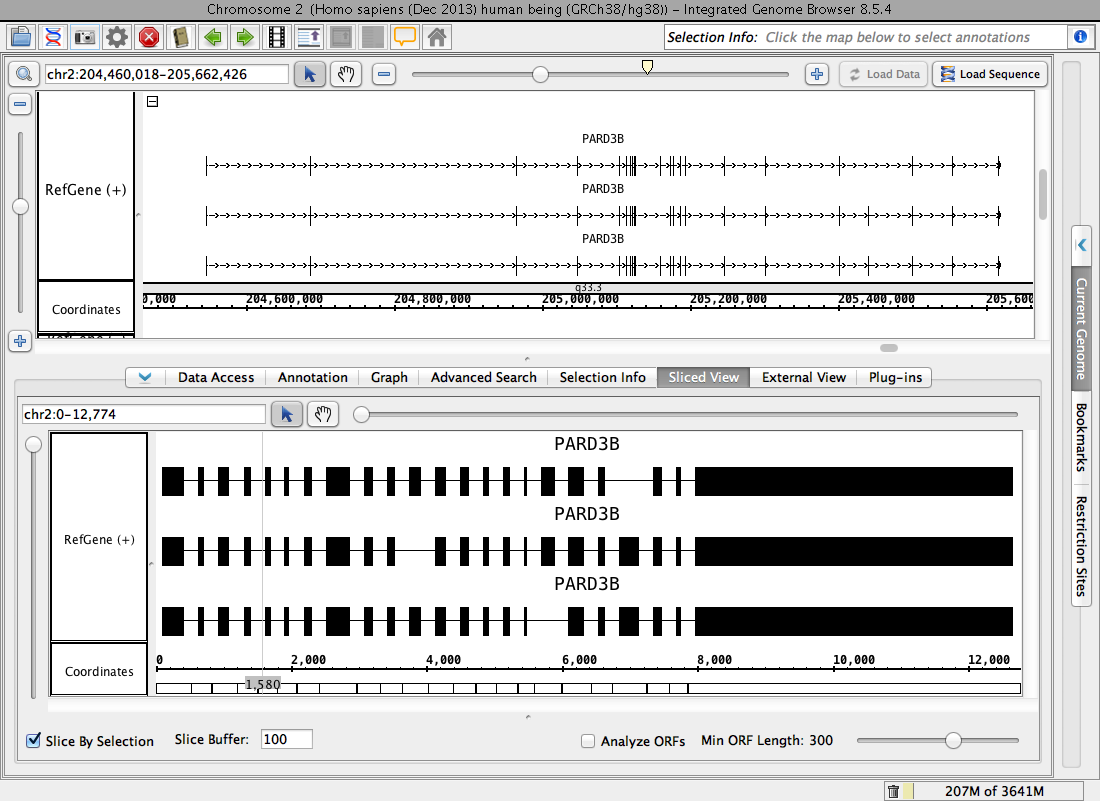
\includegraphics[width=1\textwidth]{img/browser-igb.png}
		\caption{Przeglądarka IGB.}
		\vspace{-0.5cm}
		\caption*{\scriptsize Źródło: \url{http://bioviz.org/igb/less/images/SlicedView.png}}
		\label{img:przegladarka-igb}
	\end{figure}
	
\subsection*{Inne narzędzia}	
	\item \emph{Alamut} \label{alamut} \\
	%http://www.interactive-biosoftware.com/
	przeglądarka oferująca jedynie ludzki genom;
	projekt zamknięty, rozwijany komercyjnie przez firmę \textit{Interactive Biosoftware}; 
	ostatnie wiadomości odnośnie rozwoju projektu z początku 2016 roku\footnote{\url{http://www.interactive-biosoftware.com/media-center/news/}}
	
	\item \emph{Argo Genome Browser} \label{argo-genome-browser} \\
	%http://www.broadinstitute.org/annotation/argo/
	opracowana na \textit{MIT} w \textit{Broad Institute}, który został powołany do życia w 2004 roku. 
	Przeglądarka napisana w języku \textit{Java 1.4}, aktualnie niewspierana - ostatnia wersja wydana na początku 2010 roku. Brak algorytmów KMP, Smitha-Watermana.
	
	\item \emph{ChIPMonk}\\
	%http://www.bioinformatics.babraham.ac.uk/projects/chipmonk/
	projekt opracowany przez \textit{Babraham Bioinformatics} na Uniwersytecie Cambridge, napisany w języku Java, ostatnie wydanie w 2011 roku, oficjalnie przestał być rozwijany.
		
	\item \emph{Biodalliance}\\
	%http://www.biodalliance.org/
	przeglądarka podobna do Ensembl, UCSC czy GBrowse. 
	Wyróżnia się implementacją w nowoczesnych webowych standardach (\textit{HTML5}), uruchamiana w środowisku przeglądarki internetowej. 
	Aktywnie rozwijana, nie wymaga części serwerowej do użytkowania. 
	Brak narzędzi do przeszukiwania genomu w celu znalezienia podobnych sekwencji.
	
	\item \href{https://www.dnanexus.com/genomes/hg18/public_browse}{\emph{DNAnexus}} \label{dnanexus} - przeglądarka do wizualizacji danych korzysta z~technologii \emph{Flash}. Jest narzędziem nowej generacji, mocno rozbudowanym w~kategorii analizy i~obrazowania sekwencji.
	
	\item \href{http://download.cnet.com/GeneWall-Genome-Browser-Pro/3000-2129_4-75855506.html}{\emph{GeneWall}} \label{genewall} - przeglądarka genomów przeznaczona na urządzenia mobilne. W~wersji podstawowej można przeglądać jedynie genom człowieka, natomiast w~wariancie profesjonalnym aplikacji mamy możliwość uploadu własnych plików z~danymi.
	
	\item \href{http://gaggle.systemsbiology.net/docs/geese/genomebrowser/}{\emph{Gaggle Genome Browser}} \label{gaggle} - otwarte narzędzie do mapowania mocno skondensowanych danych na współrzędne genomu. Oprogramowanie przeznaczone do obsługi dużych zbiorów danych, pozwala na łatwy import plików użytkownika. Współpracuje z~innymi bioinformatycznymi narzędziami zawartymi w~frameworku Gaggle.
	
	\item \href{https://genestack.com/}{\emph{Genestack}} \label{genestack} - internetowy, genomiczny system operacyjny. Pozwala wyszukiwać i~importować dane z~wielu publicznych baz danych. Potrafi konwertować dane wejściowe użytkowników z~wielu formatów. Udostępnia zestaw narzędzi dla programistów, do łatwego tworzenia własnych przeglądarek.
	
	\item \href{http://genomeview.org/}{\emph{GenomeView}} \label{genomeview} - samodzielna przeglądarka i~edytor genomu nowej generacji. Obecnie rozwijana przez społeczność \href{http://www.broadinstitute.org/}{Broad Insitute}. Zapewnia interaktywną wizualizację sekwencji, adnotacji, możliwość porównań na wielu poziomach, mapowań i~wielu innych. Dzięki systemowi wtyczek, istnieje możliwość rozszerzenia funkcjonalności przeglądarki.
	
	\item \href{http://www.genomemaps.org/}{\emph{GenomeMaps}} \label{genomemaps} - wysokowydajna przeglądarka z~interfejsem opartym o~HTML5 i~CSS3. W~dużej mierze implementowana z~użyciem biblioteki Javascript \href{https://github.com/opencb/jsorolla}{\mbox{\emph{JSorolla}}}. Dane pozyskuje korzystając z~usług REST bazy \href{https://github.com/opencb/cellbase/wiki}{\emph{CellBase}}. Uruchamia się we wszystkich nowszych przeglądarkach internetowych, nie wymagając od użytkownika instalacji dodatkowych komponentów.
	
	\item \href{http://www.popsci.com/science/article/2011-06/introducing-genome-wowser-ipad-app-lets-you-browse-human-genome}{\emph{Genome Wowser}} - aplikacja przeznaczona na urządzenia mobilne iPad, wydana przez CBMI (ang. Center for Biomedical Informatics) w~Szpitalu Dziecięcym w~Filadelfii. Pozwala przeglądać popularną bazę \emph{UCSC Genome Browser}.
	
	\item \href{https://hyperbrowser.uio.no/hb/}{\emph{Genomic HyperBrowser}} - jest wolnym oprogramowaniem na licencji \emph{GNU GPL v3}. Produkt skupiony głownie na analizie statystycznej elementów w~genomie. Tworzony z~wykorzystaniem platformy \href{https://en.wikipedia.org/wiki/Galaxy_(computational_biology)}{\emph{Galaxy}}.
	
	\item \href{http://wtsi-web.github.io/Genoverse/}{\emph{Genoverse}} - przenośna, konfigurowalna, przeglądarka oparta o~Javasript i~HTML5. Pozwala na eksplorację danych w~dynamiczny, interaktywny sposób. Dane są prezentowane w~przeglądarce, dzięki czemu może być łatwo instalowana na własnych stronach i~pokazywać dane z~wielu źródeł - gromadzonych online i~lokalnie.
	
	\item \href{http://genplay.einstein.yu.edu/}{\emph{GenPlay}} - szybkie i~łatwe w~użyciu narzędzie do analizy i~przetwarzania sekwencji napisane w~Javie. Uruchamia się na większości najpopularniejszych systemów operacyjnych. Prace nad projektem rozpoczęto na Kolegium Medycznym Alberta Einstein'a Uniwersytetu Yeshiva w~Nowym Yorku. Przeglądarka aktualnie w~fazie testowania, używana przez studentów.
	
	\item \href{http://img.jgi.doe.gov/}{\emph{Integrated Microbial Genomes}} - zaawansowany system wspierający analizę i~adnotacje mikrobiologicznych zbiorów danych i~metadanych genetycznych zgromadzonych w~\emph{DOE's Joint Genome Institute}. Współpracuje z~wieloma instytucjami.
	
	\item \href{http://mgv2.cmbi.ru.nl/}{\emph{Microbial Genomic Viewer}} - łatwe w~obsłudze narzędzie do interaktywnej wizualizacji wyników analizy porównawczej genomów. 
	
	\item \href{https://www.nextbio.com}{\emph{NextBio Genome Browser}} - interaktywna aplikacja pozwalająca na wizualizację zależności pomiędzy prywatnymi lub publicznymi zbiorami danych biologicznych różnych typów.
	
	\item \href{http://persephone.net/}{\emph{Persephone}} - rozbudowana aplikacja nowej generacji szeroko używana przez bioinformatyków i~genetyków. Możliwość bezpłatnego korzystania z~wersji \emph{trial} przez 30 dni.
	
	\item \href{http://www.plantgdb.org/}{\emph{PlantGDB}} - przeglądarka z~zestawem narzędzi analitycznych wraz ze zbiorami danych genetycznych wielu roślin.
	
	\item \href{http://tabit.ucsd.edu/}{\emph{STAR}} - zintegrowane środowisko do zarządzania i~wizualizacji danych sekwencjonowania. Płynność działania aplikacji w~przeglądarce internetowej zapewnia połączenie technologi JavaScript, HTML5 i~asynchronicznej komunikacji do wymiany danych. 
	
	\item \href{http://tgac-browser.tgac.ac.uk/}{\emph{TGAC Browser}} - nowa open-source'owa przeglądarka genomów obrazująca adnotacje z~bazy danych \emph{Ensembl}. Wyprodukowana przez \emph{Centrum Analizy Genomów} w~Wielkiej Brytanii (ang.\emph{The Genome Analysis Centre, UK}).
	
	\item \href{http://ugene.net/}{\emph{Ugene}} - darmowa platforma bioinformatyczna wspomagająca użytkowników w~pracach nad sekwencjami. Oferuje narzędzia do analizy danych, przypisów, porównań itp. Dane wejściowe mogą być składowane lokalnie albo udostępnione z~innych źródeł. Napisana w~C++ z~wykorzystaniem biblioteki Qt. Funkcjonuje na licencji GPL.
	
	\item \href{http://enhancer.lbl.gov/}{\emph{VISTA Enhancer Browser}} - kompleksowy zestaw baz danych, narzędzi, serwerów na potrzeby analizy porównawczej sekwencji genomów. Istnieją 2 sposoby na korzystanie z~przeglądarki: można wysyłać własne sekwencje i~dopasowania do analizy, bądź sprawdzać z~wstępnie przetworzonymi danymi całych genomów różnych gatunków. Projekt rozwijany we współpracy z~wieloma instytucjami.
	
	
\end{itemize}

\chapter{Projekt i implementacja}


\section{Architektura}

Przeglądarka została zaimplementowana w wielowarstwowej architekturze klient-serwer.
Kod został podzielony na moduły, aby jak najbardziej oddzielić od siebie niezależne fragmenty aplikacji zachowując przy tym dobre praktyki programistyczne.
Rozróżniamy w pracy 3 główne warstwy odpowiadające za:
\begin{itemize}
	\item prezentację
	\item obsługę danych
	\item logikę biznesową
\end{itemize}

\subsection*{BioWeb}

BioWeb jest środowiskiem aplikacyjnym, w którym zostało stworzonych wiele aplikacji przetwarzających dane genetyczne \cite{article:bioweb}.
Programy operujące na obszernych zbiorach genetycznych wymagają architektury zapewniającej m.in. przenośność, elastyczność i wysoką wydajność nie rezygnując jednocześnie z interaktywnego interfejsu użytkownika.
Zaspokojenie ww. wymagań możliwe jest dzięki połączeniu ze sobą w jednym projekcie języków kompilowanych i interpretowanych.
Zastosowanie architektury BioWeb przyspiesza sam proces wytwarzania oprogramowania poprzez podejście zalecające implementację jedynie modułów obliczeniowych w językach niskiego poziomu (C++), natomiast część serwerową i kliencką, które nie są wąskimi gardłami, w językach interpretowanych takich jak Python i Javascript.
Innymi słowy - moduły nie wymagające ponad przeciętnej wydajności, które można stworzyć szybciej, implementowane są w językach wyższego poziomu a moduły zasobożerne są w językach niskiego poziomu. Odpowiedni dobór konkretnych technologii dał możliwość wygodnego połączenia ww. technik.
Na rysunku \todo{[link]} zamieszony został schemat struktury aplikacji.
\\
\todo{[rysunek schematu - trójwarstwowa aplikacja ze schematem technologii.]}


\subsection*{Klient, warstwa prezentacji}
Moduł klienta znajdujący się w warstwie prezentacji możemy zaliczyć do grupy klientów cienkich.
Odpowiada on za ilustrowanie danych pobranych z serwera wykonując operacje renderowania elementów graficznych oraz zapewnia interaktywną komunikację użytkownika z systemem.
W obecnych czasach, praktycznie każdy komputer stacjonarny a nawet urządzenia mobilne posiadają stosunkowo dużą moc obliczeniową pozwalającą na proste przetwarzanie.
Realizując projekt, zastosowano podejście, w którym odpowiedzialność za operacje takie jak walidacja danych, generowanie rysunków czy animacje pozostają na barkach modułu klienckiego. 
Tym samym, odciążony zostaje serwer, przez co podwyższamy jego możliwości wydajnościowe co sprowadza się do zwiększenia potencjalnej liczby jednocześnie obsługiwanych użytkowników.

Do implementacji warstwy prezentacji zostały użyte technologie webowe, wykorzystujące jako środowisko uruchomieniowe przeglądarkę internetową. Użytkownikowi wystarczy jedynie maszyna z dostępem do internetu i nowoczesną przeglądarką internetową wpierająca HTML5. 
Klient może być uruchomiony na dowolnym popularnym systemie operacyjnym \mbox{(Linux/Mac/Windows)} i zwolniony jest z potrzeby aktualizowania aplikacji - wszystkie moduły ładowane są podczas inicjacji przeglądarki genomu.

\subsection*{Serwer - warstwa trwałości i przetwarzania}
Serwer jest przenośny, wykorzystuje technologie dające się uruchomić na najpopularniejszych platformach komputerowych - Unix, Windows.
System pozwala na równoległą obsługę wielu użytkowników jednocześnie.
W celu zwiększenia wydajności aplikacja daje się stosunkowo łatwo skalować horyzontalnie i wertykalnie.
Wpływ na szybkość przetwarzania żądań, głównie ma klasa zastosowanego sprzętu komputerowego.
Jego główne zadania to gromadzenie danych, udostępnienie ich dla aplikacji klienckiej poprzez API, przechowywanie stanu przeglądarki, wykonywanie zadań przeszukiwania genomu.

\section{Wykorzystane technologie}
Python jest głównym językiem programowania używanym w przeglądarce.
Jest interpretowany, wspiera wiele paradygmatów programowania, uważany jest jako prosty do nauki, posiada rozbudowaną bibliotekę standardową i jest mocno wspierany przez społeczność. 
Aplikacje pisane w nim są przenośne i szybkie zarazem, ponieważ wiele bibliotek pod spodem jest zaimplementowanych w C/C++.

Algorytmy do wyszukiwania sekwencji, zostały zaimplementowane w języku C++ i zintegrowane z częścią serwerową za pomocą biblioteki \textit{BoostPython}.
Biblioteka ta stworzona została aby szybko i łatwo eksportować C++ do Pythona.
Jest tak zaprojektowana, aby była minimalnie inwazyjna dla kodu C++ - w większości przypadków nie ma konieczności w żaden sposób zmieniać klas C++ aby używać ich z \textit{BoostPython}.

Aby uprościć standardowe czynności związane z pisaniem aplikacji webowej wykorzystany został popularny framework pythonowy - Django. 
Automatyzuje on wiele zadań związanych z obsługą żądań HTTP (Django REST Framework), dostarcza panel administracyjny, system cache'owania, serwer do testowania aplikacji i wiele innych.
Kluczową dostarczoną funkcjonalnością jest maper obiektowo relacyjny ORM\footnote{ang. Object Relational Mapping.}, który w wygodny sposób daje nam dostęp do danych zgromadzonych w bazie danych bez potrzeby pisania niekiedy skomplikowanych zapytań SQL.
Jako system bazodanowy użyty został PostgreSQL - jeden z najpopularniejszych systemów relacyjnych o otwartym kodzie źródłowym.

Jako serwer WWW wykorzystany został Nginx, który z Django łączy się za pośrednictwem serwera HTTP Gunicorn implementującego interfejs WSGI\footnote{ang. Web Server Gateway Interface.}.

Podstawą części wizualizacyjnej, dostarczającej graficzny interfejs użytkownika (GUI\footnote{ang. Graphical User Interface}) jest język HTML5 wraz z JavaScriptem.
Element ,,canvas'' pozwala na dynamiczne, skryptowe renderowanie kształtów i obrazów bitmapowych bez dodatkowych wtyczek - został użyty do odrysowywania głównego widoku mapy genomu.
Aby ułatwić zadania towarzyszące tworzeniu aplikacji w modelu SPA\footnote{ang. Single Page Application}, wykorzystany został framework \textit{AngularJS} oparty o wzorzec projektowy MVC\footnote{ang. Model View Controller}.
Angular jest otwartoźródłowym projektem wydanym i rozwijanym przez firmę \textit{Google}.
Bardzo pomocny przy implementacji wartwy prezentacji okazał się również framework CSS\footnote{ang. Cascading Style Sheets} \textit{Bootstrap}, który ułatwił stylizację komponentów wyświetlanych na stronie.

Fragmenty kodu odpowiedzialne za budowanie aplikacji, uruchamianie jej w różnych konfiguracjach, kompilację modułów obliczeniowych itp. wykorzystują narzędzie \textit{SCons}.
Pliki konfiguracyjne mają formę skryptów pythonowych, natomiast sama funkcjonalność narzędzia pod wieloma względami przypomina tradycyjny program powłoki systemowej, automatyzujący np. proces kompilacji programów - \textit{GNU make}.

\begin{figure}[h]
	\centering
	
\includegraphics[width=1\textwidth]{img/loga.png}
	\caption{Technologie wykorzystane w projekcie.}
	\vspace{-0.5cm}
	\label{img:technologie}
\end{figure}


\section{Struktura projektu}
\todo{todo: obrazek z drzewem projektu\\}
W niniejszym rozdziale przybliżę strukturę plików i folderów w projekcie oraz wyszczególnię ważniejsze fragmenty kodu.
Zaimplementowana aplikacja została podzielona na następujące moduły:

\subsection*{build\_tools}
Zawiera klasy wykorzystywane do budowania aplikacji, pliki konfiguracyjne:


\begin{itemize}
	\item \textit{requirements.txt} - spis bibliotek pythonowych, które zostaną zainstalowane w wyizolowanym środowisku \textit{virtualenv}.
	\todo{todo: dodać link do opisu pliku SCons}
	
	\item \textit{deploy\_conf\_files} - folder zawierający szablon pliku konfiguracyjnego serwera www \textit{nginx}, wykorzystywany przy produkcyjnym budowaniu aplikacji.
	\todo{todo: dodać link do opisu pliku SCons}
	
	\item \textit{build.AppBuilder} - klasa umożliwiająca zarządzanie plikiem konfigurującym proces budowania, tworzenie struktury folderów projektu, utworzenie środowiska \textit{virtualenv} wraz z pobraniem i zainstalowaniem niezbędnych bibliotek pythonowych, pobranie i wypakowanie plików zawierających dane dotyczące genomu ogórka, które wykorzystywane są podczas inicjacji bazy danych.
	
	\item \textit{deploy.Deployer} - klasa pozwalająca renderować plik konfiguracyjny serwera www \textit{nginx}, generować sekretny klucz \textit{Django}, konfigurować ustawienie \textit{Django ALLOWED\_HOSTS} niezbędne do prawidłowego działania serwera.
\end{itemize}

\subsection*{functional\_tests}
Zawiera sterownik do silnika przeglądarki \textit{Chrome} oraz testy funkcjonalne wykorzystujące bibliotekę do testowania webowych aplikacji - \textit{Selenium}.

\subsection*{zpr}
Zawiera główne ustawienia \textit{Django} (settings.py) oraz korzeń API HTTP aplikacji (urls.py).

\subsection*{zpr/database}
Zawiera skrypty służące do parsowania danych biologicznych pozyskanych od SGGW, narzędzia do obrabiania tych danych, tj. ekstrahowania informacji, przygotowywania struktur pomocniczych, grupowania, filtrowania, zliczania, sortowania oraz finalnie - generowania ciągów chromosomów po odrzuceniu błędnych, niespójnych danych.

\subsection*{zprapp}
Główny folder aplikacji, zawiera moduły logiki i prezentacji.
Bezpośrednio w folderze znajdują się m.in. pliki widoków API, serializerów, trasowania url, panelu administracyjnego, schematu bazy danych, testów jednostkowych.

\subsection*{zprapp/calc}
Zawiera algorytmy wyszukiwania podciągów zaimplementowane w języku \textit{C++}: \textit{Knutha-Morrisa-Pratta}, \textit{Boyera-Moore'a}, \textit{Smitha-Watermana}, \textit{BLAST} oraz ich interfejsy pozwalające na wywołanie kodu bezpośrednio z poziomu \textit{Pythona}. Algorytmy zostały zaimplementowane przez \textit{Piotra Róża}.

\subsection*{zprapp/templates/zprapp}
Zawiera pliki HTML dynamicznie renderowane w przeglądarce internetowej podczas użytkowania aplikacji.

\subsection*{zprapp/static/zprapp}
Zawiera biblioteki Javascriptowe wraz ze stylami CSS wykorzystywane po stronie frontendu.
Tutaj została zaimplementowana większość kodu kontrolerów Angularowych.
W folderze \textit{lang} obecne są również pliki zawierające tłumaczenia słów w dwóch językach - angielskim i polskim.
Aplikację w prosty, nieinwazyjny sposób można rozszerzyć o więcej języków.

\subsection*{zprapp/contrib}
Lokalizacja zawierają funkcje i klasy wykorzystywane m.in. do pomiarów i porównania szybkości algorytmów oraz łączenia ciągów podsekwencji w dłuższe fragmenty.


\section{Baza danych}

\section{Algorytmy}

\section{Sekwencje ogórka}

\section{Interfejs użytkownika}

\section{Instrukcja uruchomienia aplikacji}
W celu zautomatyzowania budowy, kompilacji oraz konfiguracji aplikacji zostało wykorzystane narzędzie \textit{Scons}.
Aby zbudować i uruchomić część serwerową przeglądarki genomów w środowisku Linux z rodziny \textit{Debian}, zaleca się wykonać następujące czynności:
\begin{enumerate}
	\item zainstalować bazę danych \textit{PostgreSQL} w wersji 9.5
	\item zainstalować język Python w wersji 2.7 wraz menadżerem paczek \textit{pip} i środowiskiem virtualenv
	\item zainstalować bibliotekę \textit{Boost} w wersji 1.64
\end{enumerate}
Powyższe zadania można wykonać poleceniami:

\begin{spverbatim}
	apt-get install libpq-dev python-dev python-pip scons postgresql nginx
	pip2 install virtualenv
	tar --bzip2 -xf /path/to/boost_1_64_0.tar.bz2 ./bootstrap.sh --with-python=python ./b2 install
\end{spverbatim}

\begin{enumerate}[resume]
	\item utworzyć użytkownika \textit{zpr} o haśle \textit{zpr}
	\item utworzyć bazy danych \textit{zpr} oraz \textit{ogorek\_roboczy}
\end{enumerate}
Powyższe zadania można wykonać poleceniami:

\begin{spverbatim}
	sudo -u postgres createuser --superuser --createdb --createrole zpr 
	sudo -u postgres psql -c "alter user zpr with encrypted password 'zpr';"
	sudo -u postgres createdb -O zpr zpr 
	sudo -u postgres createdb -O zpr ogorek_roboczy
\end{spverbatim}

\begin{enumerate}[resume]
	\item przetestować połączenie z bazą danych poleceniem\\
	\verb|psql zpr -U zpr|\\
	w przypadku pojawiającego się błędu\\
	\verb|psql: FATAL: Peer authentication failed for user "zpr""|
	należy w pliku \textit{/etc/postgresql/9.5/main/pg\_hba.conf} w linijce \textit{local all all peer} zamienić \textit{peer} na \textit{md5}, następnie zrestartuj serwer poleceniem\\
	\verb|#/etc/init.d/postgresql restart|
	
	\item zbudować program wraz ze środowiskiem poleceniem \verb|scons|
	
	\item wczytać bazę danych \textit{ogorek\_roboczy} poleceniem\\
	\verb|scons restore_ogorek_roboczy=1|
	
	\item zbudować główną bazę danych poleceniem \verb|scons build_db=1|
	
	\item w celu konfiguracji produkcyjnej serwera www \textit{nginx} wykonać:\\
	\verb|sudo scons build_deploy=1|\\
	Należy pamiętać aby w pliku \textit{SConstruct} ustawić odpowiednio zmienne, w szczególności \textit{WWW\_SRV\_HOST}.
	W razie błędu \textit{HTTP 400}, należy sprawdzić czy w pliku \textit{settings.py}, w zmiennej \textit{ALLOWED\_HOSTS} jest prawidłowo wpisana wartość \textit{WWW\_SRV\_HOST}.
	
	\item wygenerować nowy klucz zabezpieczeń \textit{Django} poleceniem:
	\verb|new_secret_key=1|\\
	Klucz powinien pozostać taki sam w poszczególnych wdrożeniach.
	
	\item uruchomić serwer lokalnie bądź produkcyjnie poleceniami odpowiednio:\\
	\verb|scons run=l| lub \verb|scons run=p|\\
	Jeśli serwer www nie serwuje prawidłowo plików statycznych należy sprawdzić uprawnienia dostępu do folderu \textit{static}
\end{enumerate}







\chapter{Wyniki}

\section{Baza danych}
-znaczenie danych

\section{Sekwencje ogórka}
\todo{tabela z wynikami \ref{tab:genome_stat}}

\begin{table}
	\centering
	\begin{tabular}{|c||r|r|r|c|} \hline
		\textbf{Chromosom}    & Długość [Mbp] & Liczba & Zmapowana & Zmapowana \\
		& & zmapowanych contigów & długość [bp] & długość [\%] \\
		\hline
		\textbf{1}             & 55                 &  22                 &  32970425          & 59.9\%               \\
		\textbf{2}             & 44                 &  13                 &  23992470          & 52.2\%               \\
		\textbf{3}             & 65                 &  14                 &  39532546          & 60.8\%               \\
		\textbf{4}             & 61                 &  15                 &  24781874          & 40.6\%               \\
		\textbf{5}             & 49                 &  22                 &  26573846          & 54.2\%               \\
		\textbf{6}             & 42                 &  19                 &  29507078          & 70.2\%               \\
		\textbf{7}             & 52                 &  11                 &  18951584          & 36.4\%               \\
		\hline
		$\mathbf{\Sigma}$      &368                 & 116                 & 196309823          &  53.3\%              \\
		\hline
	\end{tabular}
	\caption{Chromosome statistic for mapped contigs of Nothern European cucumber genome.
		The length of the chromosomes and length of the genome described in~Chen's studies\cite{article:reevaluation_in_cucumber} was used.}
	\label{tab:genome_stat}
\end{table}

\section{API}

\section{Algorytmy}
Porównanie ze sobą dwóch sekwencji nie może polegać na zwykłej analizie ciągów tekstowych, ponieważ porównując ciągi musimy brać pod uwagę ich podłoże ewolucyjne. Chcemy sprawdzić na ile podobna jest jedna sekwencja do drugiej, analizując możliwość ewolucyjnego przekształcenia pierwszej w drugą. 
\todo{porównanie, komentarz}

\begin{figure}[h]
	\centering
	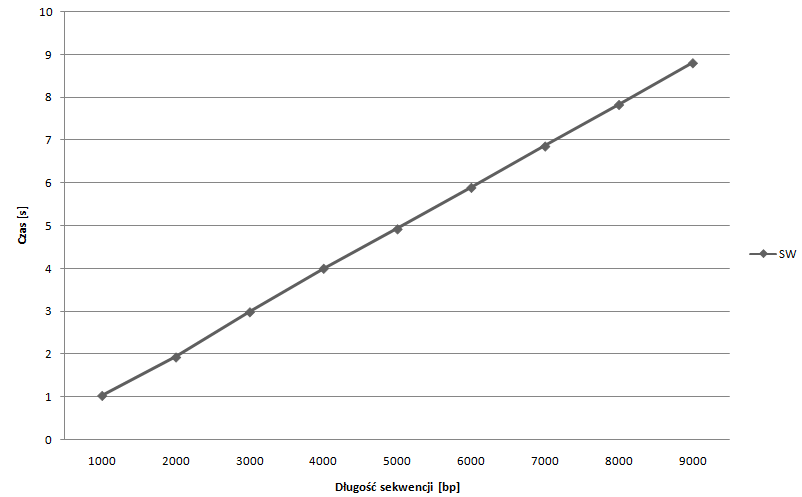
\includegraphics[width=1\textwidth]{img/sm-sekwencja-zmienna.png}
	\caption{\todo{opis - zmienna sekwencja}}
	\label{img:sm-sekwencja-zmienna}
\end{figure}

\begin{figure}[h]
	\centering
	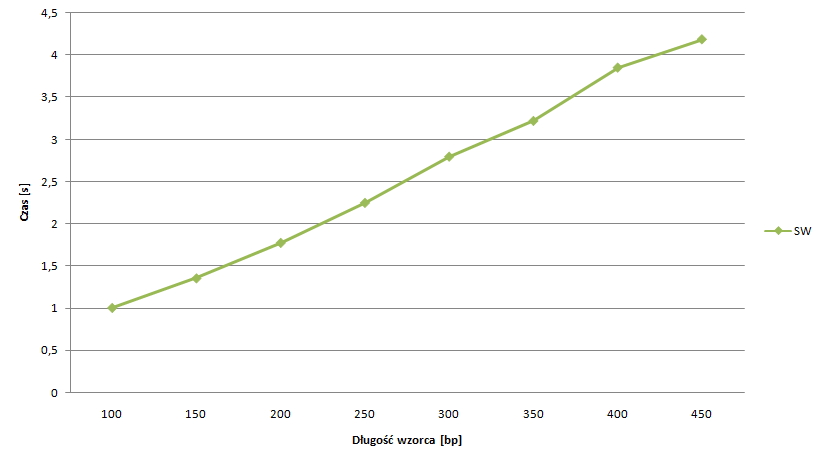
\includegraphics[width=1\textwidth]{img/sm-wzorzec-zmienny.png}
	\caption{\todo{opis - zmienny wzorzec}}
	\label{img:sm-wzorzec-zmienny}
\end{figure}

\begin{figure}[h]
	\centering
	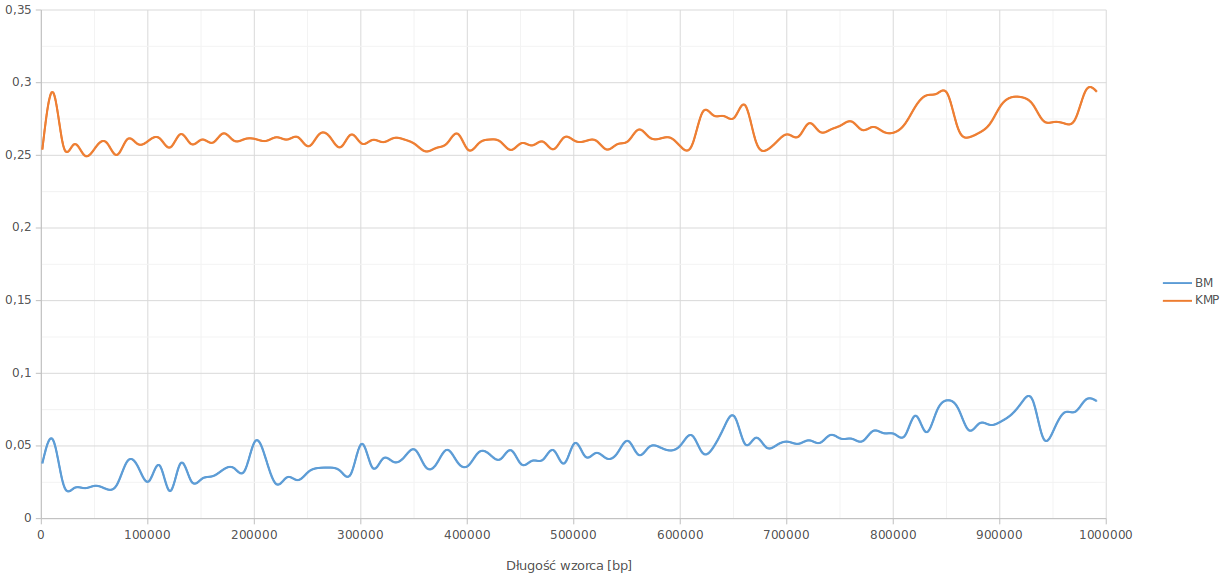
\includegraphics[width=1\textwidth]{img/kmp-vs-bm.png}
	\caption{\todo{opis - BMP vs KMP}}
	\label{img:kmp-vs-bm}
\end{figure}

\chapter{Podsumowanie}
\label{section:podsumowanie}

% \chapter{Opis algorytmów}
\label{ch:algorithms}



% \chapter{Implementacja}
\label{design}



% \chapter{Badania}
\label{section:badania}



% \chapter{Podsumowanie}
\label{summary}



\chapter*{Bibliografia}
\nocite{*}
%\bibliographystyle{plplain}
\bibliographystyle{unsrt}

%\bibliographystylebk{plplain}
%\bibliographystylest{plplain}
%\bibliographystyledoc{plplain}
% \bibliographystyleweb{plplain}
%\bibliographybk{BIB/books}
%\bibliographyst{BIB/books}
%\bibliographydoc{BIB/books}
% \bibliographyweb{BIB/books}

\bibliography{bib/mgr}

\appendix

%% \input{spis_rysunkow}

%% \input{spis_tabel}

%\input {spis_zalacznikow}

% \chapter{Instrukcje użytkownika}
\label{instructions}



\end{document}

% ex: set tabstop=4 shiftwidth=4 softtabstop=4 noexpandtab fileformat=unix filetype=tex spelllang=pl,en spell:

